% vim:spell spelllang=sk
\subsection{Spektrálna analýza}

Snáď najdôležitejšou aplikáciou fourierovej transformácie vo fyzike a
chémii je spektrálna interferometria. V tejto kapitole v skratke
rozvedieme najdôležitejšie pojmy a mechanizmy o tejto pre chemikov
životne dôležitej metóde skúmania látok.


Ako už názov naznačuje, spektrálna analýza má za úlohu analyzovať
látky. Deje sa tak prostredníctvom infračervených vĺn. Čitateľ by sa
mohol opýtať, prečo sa používajú tieto vlny a jeho zvedavosti bude za
chvíľu zadosťučinené.

\subsubsection{Chemické väzby}

Základom každej chemickej zlúčeniny sú atómy, medzi ktorými vznikajú
väzby. Väzba je akási neviditeľná pružina, ktorá vzniká ako dôsledok
pôsobenia elektromagenetickej a slabej jadrovej sily. Existuje istá
vzialenosť molekúl, keď sú tieto sily v rovnováhe a celková energia
väzby je minimálna. Vychýlením atómu zo svojej polohy prevládne jedna
z týchto dvoch síl a atóm má snahu dostať sa do svojej pôvodnej
polohy. Samozrejme, atómy za predpokladu bežnej teploty nestoja na
mieste ale kmitajú okolo rovnovážnej polohy a väzby ich držia pokope.

To čo je ale pri spektrálnej analýze dôležité je, že rôzne väzby sa
správajú rôzne. Kratšie väzby kmitajú rýchlejšie, väzba od ťažkých
atómov kmitá pomalšie, a takisto vlastnosti väzby závisia aj od
elektrických vlastností atómov. Preto sa každá väzba dá identifikovať
podľa svojej frekvencie kmitania. Prehľad niektorých vybraných typov
väzieb a k nim prislúchajúcich frekvencií sa dá nájsť v tabuľke 
\ref{tab:vazby} (čiastočne prevzaná z \cite{wiki:spectro}).
Po nahliadnutí do tabuľky by nám už malo byť jasné, odkiaľ dostala
spektrometria prívlastok infračervená - infračervené (tepelné) lúče
majú vlnovú dĺžku medzi 750nm a 1mm.

\begin{table}[htb]
    \centering
    \begin{tabular}{| l | r | r |}
        \hline
        väzba & špecifický typ väzby & vlnová dĺžka $\cm^{-1}$ \\ \hline
        C-O & alkoholy & 1040-1060, 1100 \\ \hline
        C-H & C=CH & 3020 \\ \hline
        C-H & metyl & 1260 \\ \hline
        C=O & aldehyd & 1725 \\ \hline
        C-C & aromatické C=C & 1450, 1500, 1580, 1600 \\ \hline
        O-H & alkoholy & 3200-3400 \\ \hline
        N-H & amíny & 3400-3500, 1560-1640 \\ \hline
    \end{tabular}
    \caption{Ukážka absorbčných frekvencií väzieb}\label{tab:vazby}
\end{table}

Otázkou teda ostáva, ako odhaliť frekvenciu kmitania väzieb. Odpoveď
nám núka fyzika sama. Atómy sa bežne nachádzajú v základnom stave.
Avšak pôsobením žiarenia s frekvenciou rovnou frekvencii kmitania
väzby môžeme atóm rozkmitať ešte viac. Je to jav podobný rezonancii - 
vonkajším pôsobením vynútime kmity rezonátora - väzby.
Takto rozkmitaný atóm sa môže dostať do excitovaného stavu. Pri tomto
prechode medzi stavmi atóm pohltí energiu. Zo zákona zachovania
energie musí tým pádom dopadajúce žiarenie stratiť nejakú časť
energie. No a táto strata energie (na príslušnej frekvencii) je
základom pre spektrometriu.


\begin{poznamka}
    Viac o chemických väzbách sa dá nájsť v \cite{wiki:bonds} a
    \cite{Chem}. Taktiež na stránke \cite{webspectra} sa dá nájsť
    interaktívny program na porovnávanie spektier.
\end{poznamka}

\subsubsection{Konštrukcia spektrometra}

Spektrometer môžeme rozdeliť na niekoľko základných častí.
\begin{itemize}
    \item zdroj IR žiarenia 
    \item Michaelsonov interferometer - zložený z takzvaného
    ``beamsplittera'' čo je polopriepustné zrkadlo, jedného fixného
    a jedného pohyblivého zrkadla
    \item kryštál
    \item detektor
\end{itemize}
Zjednodušenú schému spektrometra možno vidieť na obrázku
\ref{fig:ftir_schema}

\begin{figure}[htp]
    \centering
    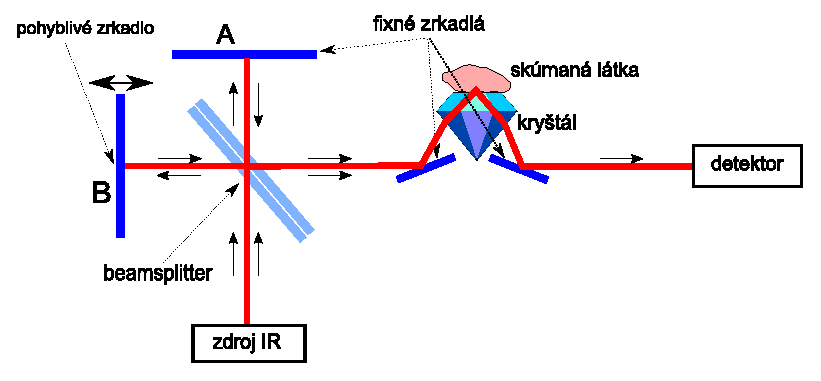
\includegraphics{obrazky/fyzika/ftir/ftir_schema}
    \caption{Základná konštrukcia spektrometra}\label{fig:ftir_schema}
\end{figure}

Infračervený lúč začne svoju púť v zdroji žiarenia. Obvylke je to 
cievka, ktorá je napájaná jednosmerným napätím a zohrieva sa.
Potom, ako lúč opustí zdroj, narazí na beamsplitter. Beamsplitter
je IR priehľadný materiál, napríklad bromid draselný (KBr). 
Beamsplitter pôsobí
na lúč ako polopriehľadné zrkadlo. Približne jednu polovicu žiarenia
prepustí smerom na zrkadlo A, druhú polovicu smerom na zrkadlo B.
Žiarenia odrazené od zrkadla A sa opäť dostáva do beamsplittera,
časť pokračuje smerom ku kryštálu a časť sa vracia do zdroja.
Žiarenie odrazené od zrkadla B sa taktiež dostáva do beamsplittera a
opäť jedna časť sa vráti do zdroja a druhá časť pokračuje v smere na
kryštál. Nás bude odteraz zaujímať iba žiarenie smerujúce do kryštálu.
Toto žiarenie je zložením dvoch lúčov z toho istého zdroja, avšak
(vďaka tomu, že zrkadlo B je pohyblivé) tieto lúče majú istý
dráhový rozdiel. Lúče preto spolu interferujú a môžeme
uvažovať, ze ďalej pokračuje len jeden výsledný lúč.
Tento je pomocou zrkadiel nasmerovaný do kryštálu. Kryštál má zaistiť,
aby sa lúč dostal do povrchovej vrstvy látky, od nej sa odrazil a
pokračoval ďalej k detektoru. V detektore sa zachytený signál
premení na elektrické napätie.


\subsubsection{Výpočet absorpcie}

\begin{definicia}[Transmitancia]
    $T=I/I_0$ je podiel prepusteného žiarenia látkou k dopadajúcemu
    žiareniu
\end{definicia}

\begin{definicia}[Absorbcia]
    Absorbciou budeme označovať logaritmickú škálu transmitancie,
    $A=-\log_{10}T$
\end{definicia}

Základom pre chemickú analýzu je graf $A(f)$ absorbcie materiálu v
závislosti od frekvencie. 

Celkovo môžeme teda písať, že $A(f) = -\log_{10} \frac{I(f)}{I_0(f)}$.
Problém ale ostáva v určovaní $I(f), I_0(f)$. Detektor totiž nevie rozlíšiť
žiarenia jednotlivých frekvencií ale mieša ich všetky dokopy.

\begin{poznamka}
    Existujú aj detektory, ktoré vedia rozlišovať intenzitu podľa
    frekvencie. Poväčšinou ale fungujú tak, že na vstupe detektora sa
    žiarenie nasmeruje do hranola, ktorý podobne ako v prípade svetla
    žiarenie rozloží na jednotlivé monochromatické časti a následne
    sa môže merať intenzita iba konkrétnej frekvencie. Základy možno
    nájsť na \cite{wiki:spectrometer} a komu by nestačilo, tak viac o tejto
    spektrometrii sa dá dočítať v \todo{}. 
\end{poznamka}



Výsledok ktorý odčítame z detektora je jediná hodnota 
$I=\int_0^\infty I(f) df$
\footnote{Presnejšie povedané výsledkom nie je intenzita ale energia.
Tieto 2 veličny sú ale priamo úmerné a tak je jednoduché určiť
"intenzitu"}.

Aby sme mohli z $I$ určiť $I(f)$, musíme použiť nasledujúci trik.

Nech $I(x)$ je hodnota nameraná detektorom, ak je zrkadlo B vo
vzdialenosti $x$ od beamsplittera. Pre našu pohodlnosť si ešte zavedieme,
že $x$ sa meria smerom zľava doprava. Ďalej nech $y$ je vzdialenosť zrkadla
A od beamsplittera a nech $I_z(f)$ je intenzita žiarenia o frekvencii
$f$ zdroja. Predpokladajme, že beamsplitter rozdelí žiarenia na 2 lúče
a po ďalšom prechode cez beamsplitter dostaneme lúče 
približne rovnakej intenzite. Môžeme písať
\begin{align}
    I_{z_1}(f,t) = a_1(f) \cos (2 \pi f (t+2x) + \phi) \\
    I_{z_2}(f,t) = a_2(f) \cos (2 \pi f (t+2y) + \phi) \\
\end{align}
kde $\phi$ je fáza vstupujúceho žiarenia do beamsplittera a $t$ je
vzdialenosť od beamsplittera v ktorej meriame požadovanú intenzitu a
$a_1,a_2$ sú konštanty kombinujúce pôvodnú intenzitu zdroja a
priepustnosť beamsplittera pre oba lúče.
Podľa lemy \ref{lema:lk_harmonickych_funkcii} môžeme tvrdiť, že
interferenctiou vznikne
\begin{equation}
    I_{z}(f,t,x) = a(f) \cos (2 \pi f (t+2x) + \psi)
\end{equation}
Potom detektor vo vzdialenosti $t$ zachytí intenzitu

\begin{align}
    I(x,t)=\int_0^\infty I_z(f,t,x) T(f) \dd f \\
    I(x,t)=\int_0^\infty T(f) a(f) \cos(2 \pi f (t + 2x) + \psi) \dd f
\end{align}
Posledná rovnica dáva ale nádej na zvrat v situácii. Pre fixné
$t$\footnote{A detektor je fo fixnej vzdialenosti} 
je to totiž Fourierova transformácia obohatená o posunutie a iné
nepríjemnosti. Faktom ale ostáva, že nie je veľký problém pár
substitúciami a rozšírením integrácie pomocou symetrie na celé $\R$
dostať štandardnú fourierovu transformáciu funkcie $I(f) = T(f) a(f)$.
Potom ale vieme spraviť spätnú transformáciu a z hodnôt $I(x)$
vypočítať $I(f)$.
\begin{poznamka}
    Jeden by mohol namietať, že nemôžeme zmerať
    $I(x)$ na celej množine $R$. Za rozumných predpokladov, akými sú
    žiarenie detektora len v istom frekvenčnom pásme,
    vieme obmedziť hranice integrácie na konečné hodnoty.
\end{poznamka}

Základom spektrálnej analýzy je teda nameranie $I(x)$ na istom
intervale a následné vypočítanie inverznej transformácie. Veľká výhoda
tejto metódy spočíva vo fakte, že jediná pohyblivá súčiastka je jedno
zrkadlo beamsplittera a teda realizácia je konštrukčne nenáročná.
Detektor navyše vieme jednoducho nakalibrovať meraním prázdnej vzorky.
